\section{Seven qubits: compatible moments and entropy}\label{sec:fqe-seven-entropy}

The four-qubit proof bounds compatible marginal moments and then converts those bounds into an entropy bound.
We follow the same strategy for seven qubits, where AME states again do not exist~\cite{HGS}.
Five-copy positivity determines the purity minimum and its equality orbit. For entropy, a majorant involving
each marginal and its spin flip gives a second five-copy certificate. The two optima occur at different
members of one icosahedral family.

\paragraph{The two optimisation problems.} A balanced cut divides the seven qubits into groups of three and four.
It suffices to consider the three-qubit side $S$, whose reduced state $\rho_S$ has eight eigenvalues. There are
$\binom73=35$ such subsets, and we average over all of them:
\[
 E_3(\psi)=\frac1{35}\sum_{|S|=3}S(\rho_S),\qquad
 \pi_3(\psi)=\frac1{35}\sum_{|S|=3}\operatorname{tr}\rho_S^2 .
\]
Every cut has entropy at most $3$ bits and purity at least $1/8$, and reaching either bound on every cut
would require an AME state.

The mean purity has a direct interpretation in terms of correlations. Expanding each marginal in Pauli strings writes $\pi_3$ as $1/8$ plus a
positively weighted sum of the squared expectation values of all Pauli strings acting on one, two or three qubits
(Appendix~\ref{sec:fqe-seven}). An AME state would make all these low-weight correlations vanish. Minimising $\pi_3$
asks how small they can be when compatibility prevents them all from vanishing. Every seven-qubit stabilizer state has
$\pi_3\ge19/140$ (Proposition~\ref{prop:stab7}), strictly above the optimum $121/917$ of
Theorem~\ref{thm:fqe-seven-purity} below; hence the purity minimiser is not a stabilizer state.

\paragraph{The two optima.} Both optimisers are members of an explicit one-parameter family of seven-qubit states
$\psi_x$, defined below. Each has one distinguished qubit $s$; the other six qubits are labelled by the six axes of an
icosahedron. A single mixing weight $x\in[0,1/2]$ parametrises the family. The purity minimiser is the
\emph{icosahedral state} $\Psiico=\psi_{37/524}$, and the entropy maximiser is $\psi_{x_*}$, where $x_*=0.0698\ldots$
is the root of equation~\eqref{eq:fqe-xstar} below.

\begin{theorem}[the seven-qubit purity minimum]\label{thm:fqe-seven-purity}
Every pure seven-qubit state satisfies $\pi_3(\psi)\ge121/917$. Equality holds if and only if $\psi$ is
equivalent to $\Psiico$ under local unitaries and permutations of the qubits.
\end{theorem}
\noindent The proof is computer-assisted: a five-copy identity verified in floating point with rigorous error bounds,
followed by an exact equality analysis. It is outlined below and given in full in Section~\ref{sec:sup-seven-purity} of
the supplement.

\begin{theorem}[seven-qubit mean-entropy maximum and equality]
\label{thm:fqe-seven-entropy}
Every pure seven-qubit state satisfies
\[
 E_3(\psi)\le E_3(\psi_{x_*})=2.965356029477675899\ldots\ \text{bits}.
\]
Equality holds if and only if $\psi$ is local-unitarily and qubit-permutation equivalent to $\psi_{x_*}$.
With fixed qubit labels, the equality set consists of exactly $42$ LU orbits.
\end{theorem}
\noindent The proof is computer-assisted: a five-copy identity verified in floating point with rigorous error bounds,
an exact certificate for the scalar majorant, Theorem~\ref{thm:fqe-seven-purity}, and an exact equality analysis. It is
outlined below and given in full in Section~\ref{sec:sup-seven-entropy} of the supplement.

At four qubits $M_4$ both minimises the summed purity $P=3\pi_2$ and maximises entropy. At seven qubits these
objectives select different states (Table~\ref{tab:fqe-seven-summary}).

\begin{table}[htbp]
\centering\small
\begin{tabular}{@{}lccp{0.3\linewidth}@{}}
\toprule
 & ideal AME value (unattainable) & optimum & optimiser \\
\midrule
$\min\pi_3$ & $0.125$ & $\dfrac{121}{917}\approx0.131952$ & $\Psiico$, unique up to local unitaries and permutations \\[2ex]
$\max E_3$ (bits) & $3$ & $2.96535602947\ldots$ & $\psi_{x_*}$, unique up to local unitaries and permutations \\
\bottomrule
\end{tabular}
\caption{Mean three-qubit purity and entropy of seven-qubit pure states. The AME values are not attained. The states
$\Psiico$ and $\psi_{x_*}$ both lie in the icosahedral family $\psi_x$ defined below.}
\label{tab:fqe-seven-summary}
\end{table}

\paragraph{An explicit state.} Label the qubits $s,0,1,\dots,5$, with $0,\dots,5$ the axes through opposite vertices of
the icosahedron. Let $e_i$ denote the six-bit string with a single
$1$ at site $i$. Set $s_{ij}=-1$ for $\{i,j\}$ an edge of the pentagon $1\!-\!3\!-\!2\!-\!4\!-\!5\!-\!1$, and
$s_{ij}=+1$ otherwise. For $0\le x\le1/2$ put $\alpha=\sqrt{(1-2x)/30}$ and (equation~\eqref{eq:ico} of
Appendix~\ref{sec:ico})
\[
\begin{aligned}
  \psi_x ={}& |0\rangle_s\Bigl(\alpha\sum_{i<j}s_{ij}|e_i+e_j\rangle + \sqrt x\,|111111\rangle\Bigr)\\
         &+ |1\rangle_s\Bigl(\sqrt x\,|000000\rangle - \alpha\sum_{i<j}s_{ij}|111111-e_i-e_j\rangle\Bigr).
\end{aligned}
\]
Every member has maximally mixed one-qubit marginals, and its three-qubit marginals fall into two spectral classes
(Theorem~\ref{thm:ico}). Writing $u=(1-2x)/30$, the $20$ marginals avoiding $s$ have eigenvalues $4u$ six times and
$3u+x$ twice; the $15$ containing $s$ have eigenvalues $8u$ once, $4u$ five times and $u+x$ twice. Consequently the mean purity $\pi_3(\psi_x)$ is an explicit quadratic in $x$, with minimum $121/917$ at
$x=37/524$: the icosahedral state $\Psiico$ (Figure~\ref{fig:fqe-icosahedral}).

\begin{figure}[tbp]
\centering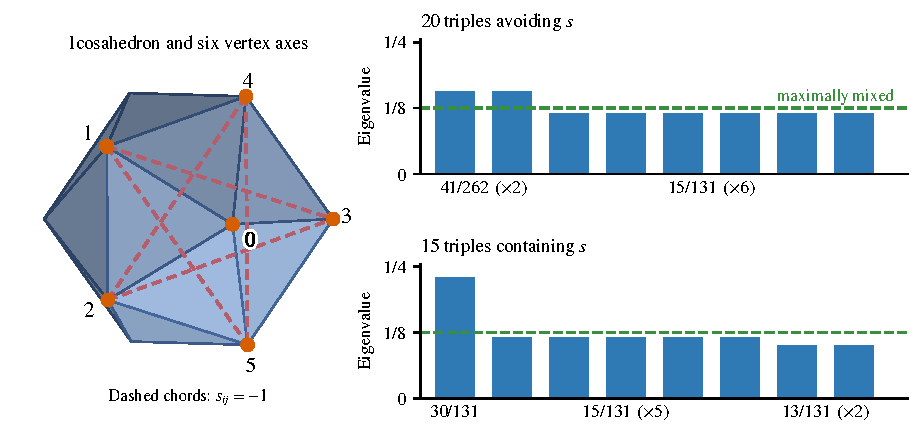
\includegraphics[width=\linewidth]{fig_icosahedron}
\caption{Icosahedral geometry and marginal spectra of $\Psiico=\psi_{37/524}$.
Left: six oriented representatives of the axes through opposite icosahedral vertices label qubits
$0,\ldots,5$; the distinguished seventh qubit $s$ is separate. Dashed chords mark pairs whose amplitude sign
$s_{ij}$ is $-1$. Right: spectra of the $20$ three-qubit marginals avoiding $s$ and the $15$ containing it;
multiplicities in parentheses (the values $(4u)^6,(3u+x)^2$ and $8u,(4u)^5,(u+x)^2$ above at $u=15/524$); every marginal in a class has the spectrum shown. The dashed horizontal line marks the maximally mixed eigenvalue
$1/8$. This state minimises the mean purity over all pure states. The entropy maximiser $\psi_{x_*}$,
$x_*=0.0698\ldots$, is a different member of the same family; its spectra have the same multiplicities, and each
eigenvalue differs from the one shown by less than $10^{-3}$, too little to see at this scale.}
\label{fig:fqe-icosahedral}
\end{figure}

The icosahedron enters through the signs. The matrix $C$ with zero diagonal and entries $s_{ij}$ off it is a symmetric
\emph{conference matrix}: $C^2=5I$. Its eigenvalues are $\pm\sqrt5$, each three times, so $I+C/\sqrt5$ is positive
semidefinite of rank three with unit diagonal. It is therefore the Gram matrix of six unit vectors in $\mathbb R^3$ with
$v_i\cdot v_j=s_{ij}/\sqrt5$: six equiangular lines~\cite{LS} at angle $\arccos(1/\sqrt5)$, which are the axes through opposite
vertices of an icosahedron. The same identity block-diagonalises every two- and three-qubit marginal of $\psi_x$ in
the computational basis, which is how Theorem~\ref{thm:ico} obtains the spectra.

The family is the fixed set of a symmetry group generated by local unitaries, qubit permutations and complex
conjugation (up to signs and phase). Hence a member stationary within the family is stationary on the whole sphere for
the purity, the entropy or any other differentiable functional invariant under these symmetries
(Lemma~\ref{lem:seven-family-symmetric-criticality} of the supplement, which identifies the group).

\paragraph{Why an icosahedron.} An exact purity identity shows why minimising purity selects this geometry. Widen the
family: replace the pair amplitudes $\alpha s_{ij}$ of $\psi_x$ by complex numbers $t_{ij}$ in the $|0\rangle_s$ branch
and by their conjugates in the $|1\rangle_s$ branch. They form a complex symmetric $6\times6$ matrix $Q=(t_{ij})$ with
zero diagonal; put $p_i=\sum_j|t_{ij}|^2$ and $\sigma=\sum_{i<j}|t_{ij}|^2$, so normalisation is $2\sigma+2x=1$. For every
such state the weight-one and weight-three Pauli correlations on the six ordinary qubits cancel between the two branches
(Theorem~\ref{thm:spinflip-double} of the supplement), and (Theorem~\ref{thm:complexsos} of the supplement)
\begin{equation}\label{eq:fqe-complex-sos}
\begin{aligned}
 \pi_3-\frac{121}{917}={}&\frac{(524x-37)^2}{137550}+\frac4{35}\sum_i\Bigl(p_i-\frac\sigma3\Bigr)^2\\
 &+\frac{48}{35}\sum_{i<j}\Bigl(|t_{ij}|^2-\frac\sigma{15}\Bigr)^2+\frac{24}{35}\sum_{i<j}\bigl|(QQ^\dagger)_{ij}\bigr|^2.
\end{aligned}
\end{equation}
At equality $x=37/524$, all $|t_{ij}|$ are equal and the rows of $Q$ are orthogonal: $Q$ is a multiple of a complex
conference matrix of order six, which is unique up to diagonal phases and permutations
(Proposition~\ref{prop:confphase} of the supplement) and is the icosahedral sign pattern above. Minimum purity thus
forces the six rows of pair amplitudes to be orthogonal with equal moduli. The identity is exact only within this
family and does not bound arbitrary states; the global bound is the five-copy certificate of
Theorem~\ref{thm:fqe-seven-purity}, whose equality analysis reduces an arbitrary minimiser to this family and this identity.

\paragraph{Entropy selects a different state.} Since the marginal eigenvalues of $\psi_x$ are affine in $x$, its mean entropy
is explicit: with $f(t)=-t\log_2t$ and $u=(1-2x)/30$,
\[
 E_3(\psi_x)=\tfrac1{35}\bigl[195f(4u)+40f(3u+x)+15f(8u)+30f(u+x)\bigr]
\]
(Appendix~\ref{sec:ico}). It is strictly concave in $x$, and its unique maximum occurs at the root $x_*\in(0,1/2)$ of
\begin{equation}\label{eq:fqe-xstar}
 2^{32}(1-2x)^{15}=3^8(1+8x)^8(1+28x)^7
\end{equation}
(Proposition~\ref{prop:entropy-seven-stationarity} of the supplement),
giving $E_3(\psi_{x_*})=2.965356029\ldots$ bits. This root lies strictly below $37/524$
(Corollary~\ref{cor:ico-entropy-separation}), so $\Psiico$ is not stationary for the entropy, even within the family.
By Theorem~\ref{thm:fqe-seven-purity} no purity minimiser maximises the mean entropy: unlike at four qubits, the two
problems have different solutions. Their objective values are nevertheless very close: $E_3(\Psiico)$ lies only $7.1597\ldots\cdot10^{-6}$ bits
below the maximum, and $\pi_3(\psi_{x_*})$ exceeds $121/917$ by $1.2204\ldots\cdot10^{-6}$ (rigorous interval enclosures).

The marginal moments give a heuristic explanation for this difference; the exact derivative in
Corollary~\ref{cor:ico-entropy-separation} supplies the proof. In the Taylor expansion of $f$ about the mean eigenvalue $1/8$,
the second-moment contribution favours small $\pi_3$, while the positive cubic coefficient favours a large
$b_3=\tfrac1{35}\sum_{|S|=3}\operatorname{tr}\rho_S^3$. At four qubits $M_4$ does both: it minimises $P$ and maximises
the cubic moment $T$ on the slice $P=1$ (Theorem~\ref{thm:fqe-moment}). Along $\psi_x$, instead,
$b_3(\psi_x)=(35008x^3+17328x^2-3084x+709)/31500$ has $b_3'(37/524)=-432/120127<0$ (Appendix~\ref{sec:ico}): moving
$x$ below $37/524$ raises $b_3$ at first order and costs $\pi_3$ only at second order.

The marginal spectra and pair purities of the minimiser agree, to the six digits published, with
those of a seven-qubit state found numerically by Di~Martino, Facchi and Florio~\cite{DMFF18}. This suggests that the two
states are LU-equivalent (Appendix~\ref{sec:ico}); Theorem~\ref{thm:ico} gives an explicit closed-form state.

\paragraph{Copies of the state.} A purity is an expectation value in two copies, and a homogeneous polynomial of
degree $m$ in $|\psi\rangle\langle\psi|$ is an expectation value in $m$ copies. Averaging the projector onto
$\psi^{\otimes m}$ over local unitaries, qubit permutations and complex conjugation gives the \emph{twirled $m$-copy
moment}. Replacing some copies by the spin-flipped state $\tilde\psi=\epsilon^{\otimes n}\bar\psi$ (which differs from $\sigma_y^{\otimes n}\bar\psi$ only by the phase $i^n$),
$\epsilon=i\sigma_y$, gives further positive operators, all linear images of it. Minimising $\pi_3$ over all moment operators subject to these positivity conditions gives lower bounds
that increase with $m$ to the true minimum, a bosonic-extension hierarchy in the spirit of~\cite{DPS}, and close to the copy hierarchy of Yu et al.\ for the pure-state
marginal problem~\cite{YSWNG} (Appendix~\ref{sec:fqe-seven} and Theorem~\ref{thm:spinflip-ppt-hierarchy} of
the supplement). A certificate at level $m$ is an identity
\begin{center}
(objective) $-$ (bound) $=$ a sum of squared norms of linear images of $m$ copies of $\psi$, some spin flipped.
\end{center}
At four qubits $P\ge1$ follows at the two-copy level from Rains' shadow inequalities~\cite{Rains}, and the sextic
identity~\eqref{eq:fqe-remainder} is a three-copy certificate for the different objective $F$ (Appendix~\ref{sec:fqe-seven}). At seven qubits the levels separate: two copies give only the AME value $1/8$, three copies
provably cannot reach $121/917$, four copies provably fall short (numerically by about $7.5\cdot10^{-5}$), and five copies are the first level that attains the sharp purity bound
(Table~\ref{tab:fqe-seven-levels}).

\paragraph{Proof outline for the purity minimum.} The proof has three steps; the entropy proof below repeats them at a
different point of the family.
\begin{enumerate}
\item \emph{Bound.} A five-copy identity writes $\pi_3-121/917$ as a sum of twelve terms, each the expectation value of a
positive operator in five copies of $\psi$, some of them spin flipped, averaged over local unitaries and qubit
permutations. Every term is therefore nonnegative, which gives the bound. Unlike at four qubits, the identity needs
computer assistance: floating-point linear algebra with rigorous error bounds establishes that suitable positive definite
coefficient matrices exist.
\item \emph{Equality moments.} At equality all twelve terms vanish. Their vanishing fixes the averaged five-copy moment of
$\psi$ to that of $\Psiico$ (Theorem~\ref{thm:fivecopy-family-equality} of the supplement): every conjugation-even,
permutation-invariant five-copy invariant of $\psi$ takes its icosahedral value.
\item \emph{Equality state.} A reconstruction theorem (Theorem~\ref{thm:moment-orbit-rigidity} of the supplement) then
shows that $\psi$ differs from $\Psiico$ only by local unitaries and a qubit permutation. Some of these invariants put
$\psi$ in the form of the widened family above, and the identity~\eqref{eq:fqe-complex-sos}
makes the amplitude matrix $Q$ a conference matrix.
With qubit labels fixed, the orbit of $\Psiico$ consists of $42$ LU orbits: $7$ choices of the distinguished qubit times
$6$ inequivalent sign patterns of the conference matrix.
\end{enumerate}
Appendix~\ref{sec:fqe-seven} defines the terms and records the tangent-line step, the invariants used and the sizes of the
computations; Section~\ref{sec:fivecopy} of the supplement gives the full proof.

\paragraph{Proof outline for the entropy maximum.} The proof follows the four-qubit pattern: a polynomial majorant
touching the entropy at the spectra of the maximiser, then a moment certificate. Across the 35 cuts of $\psi_{x_*}$, four
distinct eigenvalues occur. A single one-variable majorant of $-t\log_2t$ sharp on every cut would therefore touch at
four points and need degree at least seven, and hence seven copies (Proposition~\ref{prop:seven-entropy-majorant-degree}
of the supplement). We instead use each marginal $\rho_S$ together
with its spin flip $\widetilde\rho_S=\sigma_y^{\otimes3}\rho_S^T\sigma_y^{\otimes3}$, which is also the marginal of
$\tilde\psi$ on $S$; it has the spectrum of $\rho_S$ but in general different eigenvectors. At $\psi_{x_*}$ the two commute,
and their joint eigenvalue pairs $(\lambda,\mu)$ take only five values. With $u=(1-2x_*)/30$, the cut
eigenvalues of $\psi_{x_*}$ are $\nu_1=3u+x_*$, $\nu_2=8u$, $\nu_3=4u$ and $\nu_4=u+x_*$ (Theorem~\ref{thm:ico}), and the
pairs are $(\nu_3,\nu_3)$, $(\nu_1,\nu_1)$, $(\nu_4,\nu_4)$, $(\nu_2,\nu_3)$ and $(\nu_3,\nu_2)$.
A scalar inequality bounds the average entropy of two eigenvalues by a degree-five polynomial: there is a symmetric
polynomial $H(\lambda,\mu)$ of degree five majorising $\tfrac12[-\lambda\log_2\lambda-\mu\log_2\mu]$, with first-order
contact at those five pairs (Section~\ref{sec:seven-joint-analytic-proof} of the supplement proves it, with exact
one-variable sign checks). For arbitrary marginals the two eigenbases need not coincide. Their squared overlaps
nevertheless form a doubly stochastic matrix, so averaging the scalar inequality with these weights gives, with
$h_{kl}$ the coefficients of $H$,
\[
S(\rho_S)\le
\sum_{k,l}h_{kl}\operatorname{tr}(\rho_S^k\widetilde\rho_S^{\,l}),
\]
even when $\rho_S$ and $\widetilde\rho_S$ do not commute. The right side is a five-copy moment.

It suffices to bound this polynomial for states attaining or exceeding $E_3(\psi_{x_*})$, so the certificate is only
needed on a compact domain containing them, cut out by two technical restrictions (Proposition~\ref{prop:seven-competitor-band}
and Corollary~\ref{cor:seven-entropy-eigen-cap-497} of the supplement). The purity minimum and the entropy--purity slope
for eight eigenvalues give the \emph{purity band} $121/917\le\pi_3<8693/64000$, and
spin-flip compatibility between overlapping cuts caps every marginal eigenvalue at $497/1000$. On this
domain a positive five-copy identity bounds the polynomial by the candidate value $E_3(\psi_{x_*})$
(Theorem~\ref{thm:seven-entropy-localized-identity} of the supplement; Appendix~\ref{sec:fqe-seven} lists its terms).
At equality all its terms vanish, and the equality-moment argument and reconstruction
theorem used for purity identify the orbit (Theorems~\ref{thm:fivecopy-family-equality} and~\ref{thm:moment-orbit-rigidity} of the
supplement).

\paragraph{Stability.} Both optima are quadratically stable: each optimiser is a strict local optimum modulo local
unitaries and phase with an explicit quadratic basin, and compactness extends this to a global lower bound on the objective deficit by a constant
times the squared distance to the orbit under local unitaries and qubit permutations. We do not make the constant explicit (Theorems~\ref{thm:icolocal},
\ref{thm:icoquantbasin}, \ref{thm:entropy-seven-local} and~\ref{thm:entropy-seven-quantbasin} and
Corollary~\ref{cor:seven-global-quadratic} of the supplement).

\paragraph{Comparison with four qubits.} The two sizes differ in the equality set. At four qubits the purity minimum $P=1$ is attained on a positive-dimensional
set, containing $M_4$ and the cluster state, and the entropy needs the cut spectrum to single out $M_4$
(Proposition~\ref{prop:fqe-onecut}). At seven qubits the purity alone selects a single orbit under LU and qubit permutations,
and the two-copy level of the hierarchy is no longer sharp (Section~\ref{sec:fqe-discussion} compares other sizes).

Table~\ref{tab:fqe-four-seven} summarises the common method and the additional constraints needed at seven qubits. The degree rule of
Section~\ref{sec:fqe-entropy_maximum-entropy-bound} explains both majorants: $k=2$ gives the cubic of Section~\ref{sec:fqe-entropy_maximum-entropy-bound}, and the joint
majorant evades $k=4$ by adding the spin-flip variable. It also shows that degree five is the least possible for a joint
majorant. A joint majorant sharp at $\psi_{x_*}$ must touch at the three diagonal pairs $(\lambda,\lambda)$ among its
contacts. On the diagonal it is therefore a majorant of $-t\log_2t$ touching at three distinct points, which needs degree at least five
(Corollary~\ref{cor:seven-joint-degree-five} of the supplement). Within this majorant method five copies are therefore necessary for the entropy; that says nothing about other certificates.

\begin{table}[ht]
\centering\small
\renewcommand{\arraystretch}{1.15}
\begin{tabular}{@{}lll@{}}
\toprule
 & four qubits, $2|2$ cuts & seven qubits, $3|4$ cuts\\
\midrule
mean purity minimum & $\pi_2=1/3$ (two copies) & $\pi_3=121/917$ (five copies)\\
purity equality set & positive-dimensional, contains $M_4$ & one orbit, $\Psiico$\\
entropy maximiser & $M_4$ & $\psi_{x_*}\ne\Psiico$\\
majorant & cubic in $\lambda$, contacts $1/6,1/2$ & degree five in $(\lambda,\mu)$, five contact pairs\\
moment certificate & sextic identity, three copies & certified identity, five copies\\
extra constraints & none & purity band, cap $\lambda\le497/1000$\\
entropy equality & $M_4$ orbit (Theorem~\ref{thm:fqe-entropy-max}) & $\psi_{x_*}$ orbit\\
\bottomrule
\end{tabular}
\caption{The copy-hierarchy method at four and seven qubits. Here $\pi_2=P/3$ and $\pi_3$ are the mean balanced cut
purities. Orbits include local unitaries and qubit permutations; $\mu$ is an eigenvalue of the spin-flipped marginal.}
\label{tab:fqe-four-seven}
\end{table}
